%*****************************************
\chapter{Research Design}\label{04:design}
%*****************************************
%TODO Status: Glossary and bibliography checked

\section{Introduction}

A research project always starts with someone who is curious about something observed. A grocery store clerk notices that cereal in red boxes seems to come through the checkout line more frequently than cereal in blue boxes and wonders why. An economist notices that during certain times of the year the motels seem to be full when other times they are not and wonders what causes that pattern. A driver on a delivery service wonders if there is a more efficient route for the daily deliveries.

Researchers typically ``start where they are,'' an idea eloquently described by Kristin Esterberg\cite{esterberg2002qualitative}, who stated, ``Instead of thinking of yourself as a neutral, disinterested observer, think about the connections that you bring to what you plan to study.'' Whether it was thinking about a question they had pondered for some time, identifying a question about their own interests and hobbies, or taking a look at patterns in their everyday life, every researcher identifies a research question that was interesting and then collect and analyze data that helped answer that question. This chapter concerns creating a worthwhile question and planning a research project. Later chapters are devoted to collecting and analyzing data to answer a question.

Once researchers become curious about some topic of interest they must determine how they feel about the topic. An honest introspection is in order as they ask themselves what they may already believe about the topic and whether they believe that their perspective is the only valid one. If they determine that they have a preconceived notion that they think is the wisest perspective then that could be a problem. Researchers must also consider how they would react if their research proves them wrong about some believe. If they would be comfortable examining, and perhaps changing, what may be cherished notions based on their research then that is one thing, but if they would deny the research, hide the outcomes, or even change the data, then that would be a different problem altogether. Of course, just because a researcher feels strongly about a topic does not mean that it should be avoided; sometimes, the best topics to research are those about which someone feels strongly. 

Researchers who are prepared to accept all findings, even those that may be unflattering or challenging, may want to intentionally study a topic that evokes strong feelings. Sociology professor Kathleen Blee\cite{blee2005racial} has taken this route in her research. She studies hate movement participants and the people whose racist ideologies she does not share. Blee's research is successful because she was willing to report her findings and observations honestly, even those with which she may have personally taken strong issue.

One final step at this first stage is for researchers to think about what they already know about the topic of interest. There are many sources of knowledge, some are more prone to creating bias than others. For example, researchers may know of a topic from family history, a television program, or through casual conversations with friends. These could all introduce bias in the researcher's mind and it is important that researchers think about how they know what they know to help identify and correct biases that they may bring to the research project.

The purpose of this chapter is to outline a process that can be used to design a research project. To be sure, this is not the only possible way to design research, in fact, it may not even be the best way for a given research project, but it would work as a starting point for many research investigations.

\section{First Considerations}

Before starting the research design process, it would be helpful for the researcher to consider certain philosophical aspects of the project. While a failure to consider these items would not doom a research project, making these decisions early on may help to avoid messy re-starts. 

\subsection{Exploration, Description, Explanation}

Three general types of research are \gls{exploratoryresearch}, \gls{descriptiveresearch}, and \gls{explanatoryresearch}. Researchers conducting exploratory research are typically at the early stages of examining a topic. Exploratory research is often designed to determine the feasibility a more extensive study. Descriptive research describes or defines a particular phenomenon. As an example, an economist publishing the gasoline prices in various parts of a city is conducting descriptive research. Finally, research that answers ``why'' questions is referred to as explanatory research. In this case, the researcher is trying to identify the causes and effects of an observed phenomenon.

Although research can be exploratory, descriptive, or explanatory, most business research tends to be either descriptive or explanatory. Economists frequently produce research reports that describe the state of the economy without necessarily proposing some experiment to test that description. On the other hand, business and marketing research is frequently explanatory and is designed to develop concepts and theories that explain some observed phenomenon.

\subsection{Is The Topic Empirical?}

An empirical topic is one that can be investigated by observation or experience rather than one that concerns only opinions or theories. As an example, if a researcher investigated the cost of health care in order to answer the question, ``What is the best way to fund health care?'' that would not make an appropriate empirical study since the definition of ``best way'' is nebulous. The question, though, could be answered if it were re-framed a bit to simply how health care was funded then that would be a topic that could be measured and reported.

As a second example, in 2005 the Christian group \textit{Focus on the Family} denounced Spongebob Squarepants because they believe that he is a pro-gay activist as reported by David Kirkpatrick\cite{kirkpatrick2005conservatives}. Could a researcher determine if Spongebob is immoral? Of course not; this is an ethical question, not empirical. A researcher could gather facts about people's opinions concerning Spongebob and even interview the creators of the program to see what they intended, but answering the question of morality belongs to the world of ethicists or theologians, not business researchers.

\subsection{The Research Question}

Once a researcher finds a topic that is empirical then the next step is to write the research question. Following are the qualities of a good research question.

\begin{enumerate}
	\item Question. It may be rather obvious, but it must be written in the form of a question. To say that the research question is ``child-free adults'' or ``movies'' would not be a question. 
	\item Focused. A research question must be focused on one topic of interest and not something that is trying to explore many areas and hope that one of them ``sticks.''
	\item Open-ended. A research question should not be answered with a simple yes or no. For example, if a researcher asks, ``Does location influence the price of a real estate sale'' then there is nothing left to say once the ``yes'' or ``no'' answer is determined. Rather, a question like ``How does location influence the price of a real estate sale'' would be much better.
	\item Several answers. A good research question should have more than one plausible answer. If the question only has one possible answer then there is really nothing to research.
\end{enumerate}

\subsection{Hypotheses}

The purpose of \gls{positivist} research\footnote{Researchers engaged in interpretive projects may not start with a hypothesis, but one would likely be developed as the research project proceeded.} is to test a theory and in order to do that a researcher must create a \gls{hypothesis} that is derived from the theory. A hypothesis is a statement, sometimes causal, describing a researcher's expectation regarding the anticipated result of the investigation. Often, hypotheses are written to describe the expected relationship between two \glspl{variable}. Hypotheses are typically based on a theory and describe how an independent variable is expected to affect some dependent variable. If the theory accurately reflects the phenomenon it is designed to explain then the researcher's hypotheses should be verified.

As an example, Social Exchange Theory postulates, among other things, that positive outcomes from social exchanges over time increases trust and commitment\cite{lambe2001social}. A researcher may hypothesize that brand loyalty increases due to positive outcomes from social exchanges and then design some sort of investigation to test that hypothesis.

Sometimes, researchers hypothesize that a relationship will take a specific direction so an increase in one variable might lead to an increase in another; the variables are correlated. For example, a researcher may study the relationship between age and consumers' preference for sustainable products. The hypothesis may be something like ``younger consumers tend to prefer sustainable products more than older consumers.'' The research would be designed to determine if there is a difference in product preference by age. 

Note that researchers never say that they have proven a hypotheses. A statement that bold implies that a relationship has been shown to exist with absolute certainty and that there is no chance that there are conditions under which the hypothesis fail. Instead, researchers tend to say that their hypotheses have been supported (or not). This more cautious way of discussing findings allows for the possibility that new evidence or new ways of examining a relationship will be discovered. Researchers may also discuss a ``null hypothesis,'' one that predicts no relationship between the variables being studied. If a researcher ``rejects the null hypothesis,'' then it means that the variables in question are somehow related to one another.

\subsection{Feasibility}

In Chapter \ref{03:ethics}, \nameref{03:ethics}, ethical considerations were discussed that may make some research projects unfeasible. Certainly, no researcher is going to design an experiment where a business enterprise would intentionally injure children in order to test some theory. There are, though, a few practical matters related to the feasibility of a study that researchers should consider before beginning a project. 

Gaining unfettered access to a population could be problematic. For example, a project that included exploring the day-to-day experiences of maximum security prisoners may not be feasible due to the limited access a researcher would have to that population. On a more practical level, even research about something as common as children's behavior concerning snacks can raise interesting research issues. For example, Marshall, O'Donohoe, and Kline\cite{marshall2007families} conducted a study where they interviewed $ 8-11 $ year-old children to explore their exposure to food advertising and subsequent snack preference. While it is, generally, no trouble to find children that age to interview, there are questions about how honest children are with adults in a formal interview setting. While children do not necessarily intentionally lie, their responses to interview questions are almost certainly influenced by the fact than an adult is asking. What children say to each other during play would, no doubt, be far different from what they tell an adult during an interview. It may be impossible for an adult to ever truly enter the world of a child to observe what they say and do. 

Another consideration would be the limits imposed by time. Suppose a researcher wants to investigate how shopping habits change in a community that is becoming gentrified. Sullivan\cite{sullivan2014food} conducted surveys to determine the demographic characteristics of shoppers who were purchasing organic food in gentrified neighborhood. Bridge and Dowling\cite{bridge2001microgeographies} considered gentrification from the perspective of the retail landscape in several gentrified neighborhoods. However, to understand the \textit{change} that gentrification brings a researcher may need to observe a neighborhood for many years and record the demographics of the families who are shopping, interview them to find out what they are thinking and experiencing, and even analyze what they purchase. Unfortunately, researchers rarely have decades to devote to a single project so this type of longitudinal study becomes unfeasible.

The funding available for a study is also potentially limiting. Medical research often requires the use of very expensive equipment, like particle accelerators (more than \$100 million), Computerized Axial Tomography (CAT) Scanners (up to \$2.5 million), and Magnetic Resonance Imaging machines(about \$1 million). Even surveys that use equipment no more expensive than paper and pencil require researchers to spend time interviewing shoppers. If the research project involves a team of survey-takers fanning out over a wide geographic ares over several weeks then the personnel cost could easily top \$100 thousand. Even something as inexpensive as offering a participant a cup of coffee during an interview has a small, but quantifiable, cost that must be met.

In sum, the feasibility of a research project must be considered when deciding how to complete the project, or even if the project can be completed at all.

\subsection{Idiographic or Nomothetic?}

In general terms, research can be described as \gls{idiographic} or \gls{nomothetic}, as described by Joseph Ponterotto\cite{ponterotto2005qualitative}. These terms derive from Kantian philosophy and are frequently found in research reports, especially in psychology and sociology. However, understanding these concepts is beneficial in the planning stage for research in any field.

\begin{itemize}
	\item Idiographic. This term comes from the Greek \textit{idios}, which refers to an individual. Idiographic research concerns a single case or entity with no expectation that the research would be applicable to a wider application. Idiographic research sacrifices breadth of application for deeper, richer understanding of a single case. Many case studies are idiographic in the sense that only a single individual or location is studied and applicability beyond that case is not reasonable. Much of the small business research being done is idiographic in nature.
	\item Nomothetic. This term comes from the Greek \textit{nomos}, which refers to the traditional social norm. The goal of nomothetic research is to predict or explain general phenomena found in a population rather than a single case. Nomothetic research sacrifices understanding of single cases for a broader application across an entire industry. Much economic research is nomothetic in nature since it attempts to explain broad trends in an entire population. For example, an economist may predict that the economy will begin to improve but that does not guarantee that a specific business will benefit.
\end{itemize}

\subsection{Applied or Basic?}

The contribution that researchers hope to make to the body of knowledge depends on whether they are conducting \gls{appliedresearch} or \gls{basicresearch}. Applied research can be immediately applied to a specific case. Applied research would help a small business owner made changes in advertising that would improve the number of customers entering the store. Basic research, on the other hand, is designed to create, or validate, theories and would be useful to a legislator considering some change in the business laws of a state.

\subsection{Units of Analysis}

Another point to consider when designing a research project, and which might differ slightly in \gls{qualitativeresearch} and \gls{quantitativeresearch}, has to do with units of observation and units of analysis. These two items concern what the researcher observes in the course of data collection and what can later be said about those observations. A unit of observation is the item (or items) that are actually observed, measured, or collected in the course of of the research study. A unit of analysis is the entity that is reported at the end of the study, or the ``main focus'' of the study. In a given study, the unit of observation might be the same as the unit of analysis, but that is not always the case. What is required, however, is for researchers to be clear about how they define their units of observation and analysis, both to themselves and to their audiences.

As an example, one common unit of analysis is an individual. A research project designed to look at the shopping habits of people would use the individual as the unit of analysis. Market basket research, where the content of a shopper's basket is analyzed, uses the individual as the unit of analysis. A researcher may be interested in how some particular product makes a person feel or what thought process someone used to select a given product. One example of an individual unit of analysis can be found in investigating the role of social marketing on sales and services, as investigated by Alan Bright\cite{bright2000role} and Philip Kotler\cite{kotler1989social}.

A second common unit of analysis is groups. Groups, of course, vary in size and almost no group is too small or too large to be of interest to researchers. Families, friendship groups, and civic clubs (like \textit{Rotary}) are a few common groups examined by researchers. As examples, researchers might study how norms of workplace behavior vary across professions or how children's sporting clubs are organized. A rich and vast body of research has been done on small businesses and this would be using a group unit of analysis\cite{yusuf1995critical}\cite{huck1991competencies}.

Organizations are yet another potential unit of analysis that researchers might wish to say something about. Organizations are large groups where the members are not necessarily as homogeneous as in a small group and includes entities like corporations, colleges and universities, and even night clubs.

As examples, researchers might study the economic impact of globalization or how unions influence the behavior of industry leadership, as researched by Diana Hechavarria\cite{hechavarria2009cultural} and Randall Schuler\cite{schuler1998understanding}.

Social phenomena are a potential unit of analysis. Social phenomena such as voting and even cell phone app use or misuse would be phenomena that could be researched.

Finally, researchers examine policies and principles in businesses and those are typically contained in documents. In this case, then, the unit of observation would be a document while the unit of analysis is the business. This is also a good example of where the unit of observation and unit of analysis are different.

In sum, there are many potential units of analysis that a sociologist might examine, but some of the most common include:

\begin{enumerate}
	\item Individuals
	\item Groups
	\item Organizations
	\item Social phenomena
	\item Policies and principles
\end{enumerate}

There are also many topics that could be studied from more than one level of analysis, though that would become a more complex study. As an example, Kuruvilla and Ranganathan researched the way micro and macro human resource policies influenced economic development strategy in India\cite{kuruvilla2008economic}.

\section{The Research Process}\label{04:process}

Broadly speaking, research methods can be grouped into two broad categories: \gls{positivism} and \gls{interpretivism}. 
% TODO Can you come up with a graphic to compare positivism and interpretivism?

\subsection{Positivism}

\begin{itemize}
	\item Goal: theory testing
	\item Methods: laboratory experiments and surveys
	\item Approach: deductive, starts from theory and generates empirical data to test the theory
	\item Data: quantitative in nature: numeric 
	\item Analysis: statistical
\end{itemize}

\subsection{Interpretivism}

\begin{itemize}
	\item Goal: theory building
	\item Methods: action research and ethnography
	\item Approach: inductive, starts from observations and generates theory
	\item Data: qualitative in nature: textural
	\item Analysis: coding
\end{itemize}

\subsection{Iterative Design}

At its core, all scientific research is an iterative process of observation, rationalization, and validation. In the observation phase, researchers observe a natural or social phenomenon, event, or behavior of interest. In the rationalization phase, they try to make sense of the observed phenomenon, event, or behavior by logically connecting the different pieces of the puzzle; which, in some cases, may lead to the construction of a theory. Finally, in the validation phase, those theories are scientifically tested using a process of data collection and analysis and that often leads to a modification of the initial theory. However, research designs vary based on whether the researcher starts at observation and attempts to generate a theory (interpretive research) or starts at a theory and attempts to validate it with observations (positivist research).

Most traditional research tends to be positivist in nature. Figure \ref{fig04.01} provides a schematic view of such a research project. This figure depicts a series of activities to be performed, categorized into three phases: exploration, research design, and research execution. \marginpar{This generalized design does not fit all research and it should be modified to fit the needs of a specific project.}

\begin{figure}[H]
	\centering
	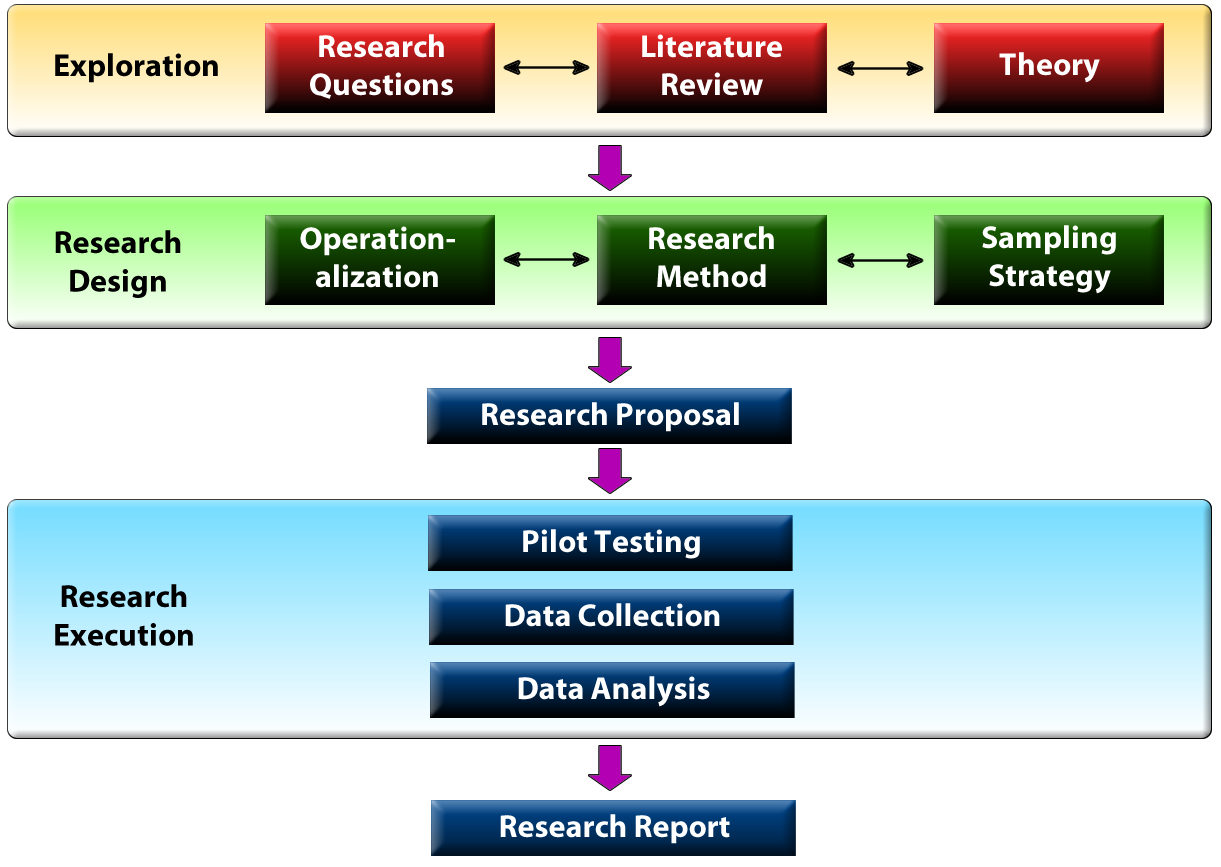
\includegraphics[width=\linewidth]{gfx/04-01}
	\caption{Positivist Research Process}
	\label{fig04.01}
\end{figure}

\begin{enumerate}
	\item \textbf{Exploration}. The first phase is exploration, which includes exploring and selecting research questions for further investigation, examining the published literature in the area of inquiry to understand the current state of knowledge in that area, and identifying theories that may help answer the research questions of interest. The diagram makes it clear that these three steps often run concurrently and researchers typically shift back-and-forth between them as needed. For example, a literature review is designed to uncover pertinent theories but finding those theories may lead to further literature review.

\begin{itemize}
	\item The first step in the exploration phase is identifying one or more research questions that deal with a specific behavior, event, or phenomena of interest. Examples include what factors motivate consumers to purchase goods and services online without knowing the vendors of these goods or services, how can high school students become more creative, and why do some people commit terrorist acts. More 	interesting research questions are those that appeal to a broader population (e.g., ``how can firms innovate'' is a more interesting research question than ``how can Chinese firms innovate in the service-sector''), address real and complex problems (in contrast to hypothetical problems), and where the answers are not obvious. Narrowly focused research questions (often with only a \textit{yes/no} answer) tend to be less useful and interesting, and generally lead to unpublishable research findings.

	\item The next step is to conduct a literature review of the domain of interest. The purpose of a literature review is three-fold: 1) to survey the current state of knowledge in the area of inquiry, 2) to identify key authors, articles, theories, and findings in that area, and 3) to identify gaps in the knowledge that a research project may be able to fill. \marginpar{Literature review is commonly done using searches in online databases.} Once a shortlist of relevant articles is generated from a search the researcher must then manually browse through each article, or at least its abstract, to determine the suitability of that article for a detailed review. Literature reviews should be reasonably complete and not restricted to only a few journals, a few years, or a specific methodology. Reviewed articles may be summarized in the form of tables and can be further structured using organizing frameworks such as a concept matrix. A well-conducted literature review should indicate whether the initial research questions have already been addressed in the literature (which would obviate the	need to study them again), whether there are newer or more interesting research questions available, and whether the original research questions should be modified or changed in light of findings of the literature review. The review can also provide some intuitions or potential answers to the questions of interest and/or help identify theories that have previously been	used to address similar questions. Reading scholarly literature is different from reading a textbook or novel. Scholarly literature is typically divided into predictable sections. One of the easiest to find is the abstract, which is a short paragraph at the beginning of an article that summarizes the research question, methods used to answer the question, and key findings. The abstract often shows whether the article is relevant to the research project. Most scholarly articles contain these sections: introduction, literature review, methodology, findings, and discussion. After the abstract, reading the discussion section is usually the next most productive. Finally, the methodology section may include important clues about a productive way to approach a research project.
	
	\item Since positivist research involves theory-testing, the third step is to	identify one or more \glspl{theory} that can help address the desired research questions. While the literature review may uncover a wide range of concepts or \glspl{construct} potentially related to the phenomenon of interest, a theory will help identify which of these constructs is logically relevant to the target phenomenon and how. Failing to identify related theories may result in measuring a wide range of less relevant, or even irrelevant constructs, while also minimizing the chances of obtaining results that are meaningful. In positivist research, theories can be used as the logical basis for postulating \glspl{hypothesis} needed in a later step. Obviously, not all theories are well-suited for studying all phenomena. Theories must be carefully selected based on their fit with the target problem and the extent to which their assumptions are consistent with that of the target problem.
	
\end{itemize}

\item \textbf{Research Design}. The next phase in the research process is research design. This process creates a blueprint of research activities that will satisfactorily answer the questions identified in the exploration phase. This includes selecting a research method, operationalizing constructs of interest, and devising an appropriate sampling strategy.

\begin{itemize}
	\item \Gls{operationalization} is the process of designing precise measures for abstract theoretical constructs. This is a major problem in business and marketing research given that many of the constructs, like ``average family'' and ``organizational culture,'' are hard to define and challenging to measure. Operationalization starts with specifying an ``operational definition'' (or ``conceptualization'') of the constructs of interest. Next, the researcher searches the literature to see if there are existing measures that can be modified to measure the constructs of interest. If such measures are not available or if they reflect a different conceptualization than that intended by the researcher then new instruments may have to be designed. This can easily be a long and laborious process, with multiple rounds of pretests and modifications before the newly-designed instrument can be accepted as ``scientifically valid.''
	
	\item Simultaneously with operationalization, the researcher must also decide what research method to employ for collecting data that will address the research question. Informing this stage of the process are the answers to philosophical questions like whether the research be exploratory, descriptive, or explanatory; will the approach be interpretive or positivist; is the goal to have some direct application or contribute more generally to the field; and what unit of analysis and observation will be used. Research methods may include experimentation, surveys, case studies, and others, or combinations of several methods in order to triangulate an answer. The selected method must then be further refined, for example, surveys could be administered by mail, telephone, web, or a combination.
	
	\item Researchers must also carefully choose the target population and a sampling strategy for data collection. While selecting a sample, care should be taken to avoid a biased sample that may generate biased observations. Sampling is covered in depth in a later chapter.
	
\end{itemize}

\item \textbf{Proposal}. At this stage, it is often a good idea to write a research proposal detailing all of the decisions made in the preceding stages of the research process and the rationale behind each decision. This multi-part proposal should address the research questions being studied and why, the current state of knowledge, theories and hypotheses to be tested, how the constructs will be measured, the research method to be employed and why, and sampling strategy. Funding agencies typically require a detailed proposal in order for them to select which to fund. Even if funding is not sought for a research project, a proposal may serve as a useful vehicle for seeking feedback from other researchers and identifying potential problems with the research project before starting data collection. This initial feedback is invaluable because it is often too late to correct critical problems after data is collected in a research study.

\item \textbf{Research Execution}. Having decided who to study (subjects), what to measure (concepts), and how to collect data (research method), the researcher is now ready to proceed to the research execution phase. This includes pilot testing the measurement instruments, data collection, and data analysis.

\begin{itemize}
	\item Pilot testing is an often overlooked but extremely important part of the research process. It helps detect potential problems in the research design and instrumentation (e.g., whether survey questions are intelligible to the targeted sample), and to ensure that the measurement instruments used in the study are reliable and valid measures of the constructs of interest. The pilot sample is usually a small subset of the target population. After a successful pilot testing, the researcher may then proceed with data collection using the sampled population.
	
	\item Next comes the actual collection of data. At this phase of the investigation the researcher would conduct surveys, visit field sites, interview subjects, read corporate documents, or generate whatever other data is specified by the plan.
	
	\item Following data collection, the data are analyzed and interpreted for the purpose of drawing conclusions regarding the research questions. Depending on the type of data collected (quantitative or qualitative), data analysis may be quantitative (e.g., employ statistical techniques such as regression or structural equation modeling) or qualitative (e.g., coding or content analysis).
		
\end{itemize}

\item \textbf{Research Report}. The final phase of research involves preparing the final research report documenting the entire research process and its findings in the form of a research paper, dissertation, or monograph. The report should outline in detail all the choices made during the research process (e.g., theory used, constructs selected, measures used, research methods, sampling, etc.) and why, as well as the outcomes of each phase of the research process. The research process must be described in sufficient detail so as to allow other researchers to replicate the study, test the findings, or assess whether the inferences derived are scientifically acceptable. Research is of no value unless the process and outcomes are documented for future generations and such documentation is essential for the progress of science.
	
\end{enumerate}

\section{Mixed Methods}

Up to this point, the research design has been treated as if it is an either/or proposition. Either a research project is positivist and numeric data are gathered or it is interpretative and textural data are gathered. In truth, researchers do not necessarily have to choose one approach over another. In fact, some of the most highly regarded business and marketing investigations combine approaches in an effort to gain the most complete understanding of their topic possible. Using a combination of multiple and different research strategies is called mixed methods because the goal is to focus on ``truth'' from several different approaches.

Imagine that a researcher were interested in finding out how college students used electronic devices on campus. Instead of just conducting one type of research, maybe a survey, two research techniques could be used, a survey and individual interviews. Finally, add to the project a content analysis of campus policies and observations of students in their natural environments\footnote{For information about using a mixed method type of research design, see John Brewer\cite{brewer1989multimethod} and Charles Teddlie\cite{teddlie2006general}.}. Researchers would end up with a comprehensive understanding of how students use electronic devices on campus. The drawback, of course, is that a mixed method project requires a larger number of resources, time, and expertise to complete. Also, along with gaining the benefit of the strengths of each type of research is the potential of the combined weaknesses becoming a problem.

\section{Common Research Mistakes}

The research process is fraught with problems and pitfalls and novice researchers often find after investing substantial amounts of time and effort into a research project that their research questions were not sufficiently answered, or that the findings were not interesting enough, or that the research was not of ``acceptable'' scientific quality. Such problems typically result in research papers being rejected by journals.

\begin{itemize}
	\item Insufficiently motivated questions. Often times, researchers choose ``pet'' problems that are interesting to the individual but not to the scientific community at large, i.e., it does not generate new knowledge or insight about the phenomenon being investigated. Because the research process involves a significant investment of time and effort on the researcher's part, the researcher must be certain (and be able to convince others) that the research questions they seek to answer in fact deal with real problems (and not hypothetical problems) that affect a substantial portion of a population and has not been adequately addressed in prior research.

	\item Pursuing research fads. Another common mistake is pursuing ``popular'' topics with limited shelf life. A typical example is studying technologies or practices that are popular today but may be obsolete in just a few years (or months). Because research takes several years to complete and publish, it is possible that popular interest in these fads may die down by the time the research is completed and submitted for publication. A better strategy may be to study ``timeless'' topics that have persisted through the years.

	\item Unresearchable problems. Some research problems may not be answered adequately based on observed evidence alone or currently accepted methods and procedures. Such problems are best avoided. However, some unresearchable, ambiguously defined problems may be modified or fine tuned into well-defined and useful researchable problems.

	\item Favored research methods. Many researchers have a tendency to recast a research problem so that it is amenable to their favorite research method (\eg, survey research). This is an unfortunate trend. Research methods should be chosen to best fit a research problem, and not the other way around.

	\item Blind data mining. Some researchers have the tendency to collect data first (using instruments that are already available), and then figure out what to do with it. In reality, data collection is only one step in the long process of planning, designing, and executing research. In fact, a series of other activities are needed in a research process prior to data collection. If researchers jump into data collection without such elaborate planning, the data collected will likely be irrelevant, imperfect, or useless, and their data collection efforts may be entirely wasted. An abundance of data cannot make up for deficits in research planning and design, and, particularly, for the lack of interesting research questions.

	\item Ecological fallacy. This occurs when claims about one lower-level unit of analysis are made based on data from some higher-level unit of analysis. In many cases, this occurs when claims are made about individuals, but only group-level data have been gathered. 

	\item Reductionism. This occurs when claims about some higher-level unit of analysis are made based on data from some lower-level unit of analysis. As an example, claims about groups are made based on individual-level data.

\end{itemize}

\section{Research Designs}

As noted on page \pageref{04:process}, research designs can be classified into two categories, \gls{positivism} and \gls{interpretivism}, depending upon the researcher's background, temperament, and research goal. Positivist designs are meant for theory testing while interpretive designs are meant for theory building. Popular examples of positivist designs include experimental (both laboratory and field), surveys, secondary data analysis, and case research while interpretive designs include case research, phenomenology, and ethnography. Note that case research can be used for both theory building and theory testing, though not at the same time. Some techniques, such as focus groups, are best suited for exploratory research, others such as ethnography are best for descriptive research, and still others such as laboratory experiments are ideal for explanatory research.

\subsection{Experimental}

Experimental studies are those that are intended to test cause-effect relationships (hypotheses) in a tightly controlled setting by separating the cause from the effect in time, administering the cause to one group of subjects (the ``treatment group'') but not to another group (``control group''), and observing how the mean effects vary between subjects in these two groups. For instance, if a laboratory experiment is designed to test the efficacy of a new drug in treating a certain ailment then a random sample of people afflicted with that ailment is found and they are randomly assigned to one of two groups (treatment and control). The drug is administered to subjects in the treatment group while a placebo is given to the control group. Finally, the two groups are monitored over a period of time to see if the treatment group has a better response than the control group. More complex designs may include multiple treatment groups, such as low versus high dosage of the drug, and multiple treatments, such as combining drug administration with dietary interventions. 

In an experimental design the subjects are randomly assigned to a group. It is ideal if the researcher knows whether individuals are in the treatment or control groups but the scientists actually administering the treatment protocol are not sure if a specific subject is receiving the drug under test or a placebo. This type of design is called a ``double-blind'' study since neither the subject nor the person administering the treatment are sure if they are in the treatment group.

If random assignment is not possible for some reason then the research design becomes ``quasi-experimental.''

Experiments can be conducted in a laboratory setting such as at a university (laboratory experiments) or in a field settings such as in an organization where the phenomenon of interest is actually occurring (field experiments). Laboratory experiments allow the researcher to isolate the variables of interest and control for extraneous variables which may not be possible in field experiments. Hence, inferences drawn from laboratory experiments tend to be stronger in internal \gls{validity}\footnote{Validity is more thoroughly defined in Chapter \ref{ch05:measuring}, page \pageref{ch05:measuring}}, but those from field experiments tend to be stronger in external validity. 

Experimental data are analyzed using quantitative statistical techniques. The primary strength of the experimental design is its strong internal validity due to its ability to isolate, control, and intensively examine a small number of variables, while its primary weakness is limited external generalizability since real life is often more complex (i.e., involve more extraneous variables) than contrived lab settings. Furthermore, if the research does not identify relevant extraneous variables and control for those variables it may decrease internal validity and lead to spurious correlations.

\subsection{Surveys}

Field surveys are non-experimental designs that do not control for or manipulate independent variables or treatments but measure these variables and test their effects using statistical methods. Field surveys capture snapshots of practices, beliefs, or situations from a random sample of subjects in field settings through a survey questionnaire or, less frequently, through a structured interview. In cross-sectional field surveys, independent and dependent variables are measured at the same point in time (e.g., using a single questionnaire), while in longitudinal field surveys, dependent variables are measured at a later point in time than the independent variables. The strengths of field surveys are their external validity (since data is collected in field settings), their ability to capture and control for a large number of variables, and their ability to study a problem from multiple perspectives or using multiple theories. However, because of their non-temporal nature, internal validity (cause-effect relationships) is problematic. Surveys may also be subject to respondent biases (e.g., subjects may provide a ``socially desirable'' response rather than their true response) which further decreases internal validity.

\subsection{Secondary Data Analysis}

Secondary data analysis is analysis of data that has previously been collected and tabulated by other sources. Data sources may include government agencies (e.g. employment statistics from the U.S. Bureau of Labor Statistics), other researchers (e.g. dissertations), or publicly available third-party data (financial data from stock markets). This is in contrast to most other research designs where collecting primary data for research is part of the researcher's job. Secondary data analysis may be an effective means of research where primary data collection is too costly or unfeasible and secondary data is available at a level of analysis suitable for answering the research questions. The limitations of this design are that the data may not have been collected in a systematic or scientific manner and hence unsuitable for scientific research. Also, since the data were collected for a presumably different purpose, they may not adequately address the research questions of interest to the researcher. Finally, interval validity is problematic if the temporal precedence between cause and effect is unclear.

\subsection{Case Research}

Case research\footnote{It is important to keep in mind that case research is not the same as a business class discussing a classic Harvard Case Study. Case research is the process of actually going to a site, gathering data, and analyzing that data.} is an in-depth investigation of a problem in one or more real-life settings (case sites) over an extended period of time. Data may be collected using a combination of interviews, personal observations, and internal or external documents. Case studies can be positivist in nature (for hypotheses testing) or interpretive (for theory building). The strength of this research method is its ability to discover a wide variety of social, cultural, and political factors potentially related to the phenomenon of interest that may not be known in advance. Analysis tends to be qualitative in nature, but heavily contextualized and nuanced. Weaknesses of case research include dependence on the observational and analytical ability of the researcher, lack of control which makes it difficult to establish causality, and inability to generalize findings from a single case site to other case sites. Generalizability can be improved by comparing the analysis from other case sites in a multiple case design.

\subsection{Focus Groups}

Focus group research is a type of research that involves bringing in a small group of subjects (typically six to ten people) to one location and having them discuss a phenomenon of interest for a period of about two hours. The discussion is moderated by a trained facilitator who sets the agenda and poses an initial set of questions for participants, then ensures that ideas and experiences of all participants are recorded, and then attempts to build an understanding of the problem based on participants' comments. Internal validity cannot be established due to lack of controls and the findings may not be generalized to other settings because of small sample size. Hence, focus groups are not generally used for explanatory or descriptive research but are suited for exploratory research projects.

\subsection{Action Research}

Action research assumes that complex social phenomena are best understood by introducing interventions, or ``actions,'' into those phenomena and then observing the effects of those actions. In this method, the researcher is usually a consultant or an organizational member embedded within a social context, such as an organization, who initiates an action, such as new organizational procedures or new technologies, in response to a real problem, such as declining profitability or operational bottlenecks. The researcher's choice of actions must be based on theory, which should explain why and how such actions may cause the desired change. The researcher then observes the results of that action, modifying it as necessary, while simultaneously learning from the action and generating theoretical insights about the target problem and interventions. The initial theory is validated by the extent to which the chosen action successfully solves the target problem. Simultaneous problem solving and insight generation is the central feature that distinguishes action research from all other research methods, and hence, action research is an excellent method for bridging research and practice. This method is also suited for studying unique social problems that cannot be replicated outside that context, but it is also subject to researcher bias and subjectivity, and the generalizability of findings is often restricted to the context where the study was conducted.

\subsection{Ethnography}

Ethnography is an interpretive research design inspired by anthropology that emphasizes the concept that a phenomenon must be studied within the context of its culture. The researcher is deeply immersed in a certain culture over an extended period of time (a few months to several years) and during that period engages, observes, and records the daily life of the studied culture. The ultimate goal is a theory about the evolution and behaviors in that culture. Data are collected primarily via observational techniques, formal and informal interaction with participants in that culture, and personal field notes, while data analysis involves ``sense-making.'' The advantages of this approach are its sensitiveness to the context, the rich and nuanced understanding it generates, and minimal respondent bias. However, this is also an extremely time and resource-intensive approach, and findings are specific to a given culture and less generalizable to other cultures.

\section{Selecting the Research Design}

Researchers tend to select designs that they are most comfortable with and feel most competent to handle; but, ideally, the choice should depend on the nature of the research phenomenon being studied. In the preliminary phases of research, when the research problem is unclear and the researcher wants to scope out the nature and extent of a certain research phenomenon, a focus group (for individual unit of analysis) or a case study (for organizational unit of analysis) is an ideal strategy for exploratory research. As the research project evolves, interpretive designs, such as case research or ethnography may be useful. If a literature review finds competing theories then positivist designs such as experimental, survey, or secondary data analysis are more appropriate.

Regardless of the specific research design chosen, the researcher should attempt to collect both quantitative and qualitative data using a combination of techniques such as questionnaires, interviews, observations, documents, or secondary data. For example, even in a highly structured survey questionnaire intended to collect quantitative data, the researcher may leave room for a few open-ended questions to collect qualitative data that may generate unexpected insights not otherwise available from the structured quantitative data alone. Likewise, while case research employ mostly face-to-face interviews to collect most qualitative data, the potential and value of collecting quantitative data using a concurrent survey should not be ignored. As an example, in a study of organizational decision-making processes, the case interviewer could record numeric quantities such as how many months it took to make certain organizational decisions, how many people were involved in that decision process, and how many alternatives were considered, and those data can provide valuable insights not otherwise available from interviewees' narrative responses. Irrespective of the specific research design employed, the goal of the researcher should be to collect as much and as diverse data as possible that can help generate the best possible insights into the phenomenon of interest.

\section{Summary}\label{ch05:summary}

Lorem ipsum dolor sit amet, consectetuer adipiscing elit. Aenean commodo ligula eget dolor. Aenean massa. Cum sociis natoque penatibus et
